\section{Nützliche Resourcen}
\begin{lemma}{Integraltabelle}\\
    \resizebox*{\linewidth}{!}{
	\def\arraystretch{1.5}
	\begin{tabular}{c|c|c}
	    Funktion | f(x)                           & Ableitung | f'(x)                         & Integral | F(x)                         \\
	    \hline
	    \(1\)                                     & \(0\)                                     & \(x+C\)                                 \\
	    \hline
	    \(x\)                                     & \(1\)                                     & \(\frac{1}{2}x^2+C\)                    \\
	    \hline
	    \(\frac{1}{x}\)                           & \(-\frac{1}{x^2}\)                        & \(\ln|x|+C\)                            \\
	    \hline
	    \(x^a \: with \: a \: \in \: \mathbb{R}\) & \(ax^{a-1}\)                              & \(\frac{x^{a+1}}{a+1}+C\)               \\
	    \hline
	    \(\sin(x)\)                               & \(\cos(x)\)                               & \(-\cos(x)+C\)                          \\
	    \hline
	    \(\cos(x)\)                               & \(-\sin(x)\)                              & \(\sin(x)+C\)                           \\
	    \hline
	    \(\tan(x)\)                               & \(1+\tan^2{(x)=\frac{1}{\cos^2{(x)}}}\)   & \(-\ln|\cos(x)|+C\)                     \\
	    \hline
	    \(\cot(x)\)                               & \(-1-\cot^2{(x)}=-\frac{1}{\sin^2{(x)}}\) & \(\ln(\sin(x))+C\)                      \\
	    \hline
	    \(e^x\)                                   & \(e^x\)                                   & \(e^x+C\)                               \\
	    \hline
	    \(a^x\)                                   & \(\ln(a)\cdot a^x\)                       & \(\frac{a^x}{\ln(a)}+C\)                \\
	    \hline
	    \(\ln(x)\)                                & \(\frac{1}{x}\)                           & \(x\ln(x)-x+C\)                         \\
	    \hline
	    \(\log_a(x)\)                             & \(\frac{1}{x\ln(a)}\)                     & \(x\log_a(x)-\frac{x}{\ln(a)}+C\)       \\
	    \hline
	    \(\arcsin(x)\)                            & \(\frac{1}{\sqrt{1-x^2}}\)                & \(x\arcsin(x)+\sqrt{1-x^2}+C\)          \\
	    \hline
	    \(\arccos(x)\)                            & \(-\frac{1}{\sqrt{1-x^2}}\)               & \(x\arccos(x)-\sqrt{1-x^2}+C\)          \\
	    \hline
	    \(\arctan(x)\)                            & \(\frac{1}{1+x^2}\)                       & \(x\arctan(x)-\frac{1}{2}\ln(1+x^2)+C\) \\
	\end{tabular}
    }
\end{lemma}
\begin{lemma}{Spezielle Grenzwerte}\\
    \[n\rightarrow \infty\]
    \resizebox*{\linewidth}{!}{
	\def\arraystretch{1.5}
	\begin{tabular}{c|c|c}
	    \(\frac{1}{n}\rightarrow 0\)& \(e^n\rightarrow \infty\)&\(\frac{1}{n^k}\rightarrow 0\ \ \forall k\in
	    \mathbb{R}^+\)\\
	    \hline
	    \(c+\frac{1}{n}\rightarrow c\)&\(e^{-n}\rightarrow 0\)&\((1+n)^{\frac{1}{n}}\rightarrow 1\)\\
	    \hline
	    \(\frac{c\cdot n}{c^n}\rightarrow 0\)&\(\frac{e^n}{n^c}\rightarrow \infty\)&\(\left(1+\frac{1}{n}\right)^c
	    \rightarrow 1\)\\
	    \hline
	\(\sqrt[n]{n}=n^{\frac{1}{n}}\rightarrow 1\)&\(\frac{\sin{n}}{n}\rightarrow 0\)&\(\left(1+\frac{1}{n}\right)^n
	\rightarrow e\)\\
	\hline
	\(\sqrt[n]{n!}\rightarrow \infty\)&\(\arctan{n}\rightarrow \frac{\pi}{2}\)&\(\left(1+\frac{c}{n}\right)^n
	\rightarrow e^c\)\\
	\hline
	\(\frac{1}{n}\sqrt[n]{n!} \rightarrow \frac{1}{e}\)&\(\ln{n}\rightarrow \infty\)&\(\left(1-\frac{1}{n} \right)^n
	\rightarrow \frac{1}{e}\)\\
	\hline
	\(\frac{c^n}{n!} \rightarrow 0\)&\(\frac{\ln{n}}{n}\rightarrow 0\)&\(\left(\frac{n}{n+c}\right)^n\rightarrow
	e^{-c}\)\\
	\hline
	\(\frac{n^n}{n!}\rightarrow \infty\)&\(\frac{\log{n}}{n-1}\rightarrow 1\)& \\
	\end{tabular}
    }
    \[n^c\cdot q^n \rightarrow 0 \quad \forall c \in \mathbb{Z},0\leq q \leq 1\]
    \[n(\sqrt[n]{c}-1)\rightarrow \ln{c}\quad \forall c > 0\]
    \[n\rightarrow 0\]
    \resizebox*{\linewidth}{!}{
	\def\arraystretch{1.5}
	\begin{tabular}{c|c|c}
	    \(\ln{n}\rightarrow -\infty\)&\(\frac{\sin{n}}{n}\rightarrow 1\)&\(\frac{1}{\arctan{n}}\rightarrow 1\)\\
	    \hline
	    \(n\log{n}\rightarrow 0\)&\(\frac{\cos{(n)}-1}{n}\rightarrow 0\)&\(\frac{e^n-1}{n}\rightarrow 1\)\\
	    \hline
	    \(\frac{\log{1}-n}{n}\rightarrow -1\)&\(\frac{1}{\cos{n}}\rightarrow1\)&\(\frac{e^cn-1}{n}\rightarrow c\)\\
	    \hline 
	    \(\frac{c^n-1}{n}\rightarrow\ln{c},\forall c>0\)&\(\frac{1-\cos{n}}{n^2}\rightarrow
	    \frac{1}{2}\)&\((1+n)^{\frac{1}{n}}\rightarrow e\)\\
	\end{tabular}
    }
\end{lemma}
\columnbreak
\begin{lemma}{Ableitungsregeln}\\
    \begin{itemize}
	\item Summenregel
	    \[f(x)=g(x)+h(x) \rightarrow f'(x)=g'(x)+h'(x) \]
	\item Differenzregel
	    \[f(x)= g(x) - h(x) \rightarrow f'(x) = g'(x) - h'(x) \]
	\item Faktorregel 
	    \[f(x)=a\cdot g(x) \rightarrow f'(x)=a \cdot g'(x) \]
	\item Produktregel
	    \[f(x)=g(x)\cdot h(x) \rightarrow f'(x)=g'(x)\cdot h(x) + g(x) \cdot h'(x) \]
	\item Quotientenregel 
	    \[f(x)=\frac{g(x)}{h(x)} \rightarrow f'(x)=\frac{g'(x)\cdot h(x)-g(x)\cdot
	    h'(x)}{h^2(x)}\]
	\item Kettenregel
	    \[f(x)=g(h(x)) \rightarrow f'(x)=g'(h(x))\cdot h'\]
    \end{itemize}
\end{lemma}
\begin{lemma}{Mitternachtsformel}\\
    \[x=\frac{-b\pm\sqrt{b^2-4ac}}{2a}\]
\end{lemma}
\section{Integralrechnen}
\subsection{Stammfunktionen}
\begin{lemma}{Integrale von Linearkombinationen}\\
	Gegeben:
	\[\int{f(x)\mathrm{d}x} = F(x)+C, \quad  \int{g(x)\mathrm{d}x} = G(x)+C\]
	Das unbestimmte Integral der Linearkombination \(\lambda_1f(x) + \lambda_2g(x)\) ist:
	\[\int{(\lambda_1f(x)+\lambda_2g(x))} = \lambda_2F(x)+\lambda_2G(x)+C \quad (\lambda_1,\lambda_2 \in \mathbb{R} )\]
\end{lemma}
\begin{lemma}{Integral von verschobenen Funktionene}\\
	Gegeben:
	\[\int{f(x)\mathrm{d}x} = F(x) + C \]
	Das unbestimte integral um Betrag k in x-Richtung verschoben ist:
	\[\int{f(x-k)\mathrm{d}x}= F(x-k)+C \quad (k \in \mathbb{R}) \]
\end{lemma}
\begin{lemma}{Integrale von gestreckten Funktionen}
	Gegeben:
	\[\int{f(x)\mathrm{d}x} = F(x)+C \]
	Das unbestimmte Integral um Faktor k in x-Richtung gestreckt ist:
	\[\int{f(k\cdot x)\mathrm{d}x}= \frac{1}{k}F(k\cdot x)+C \quad (k\neq0 )\]
\end{lemma}
\subsection{Integrationsmethoden}
\begin{formula}{Partielle Integration}
	\[\int{u'(x)v(x)\mathrm{d}x} = u(x)\cdot v(x) - \int{u(x),v'(x)\mathrm{d}x} \]
\end{formula}
\begin{formula}{Partialbruchzerlegung}\\
	\begin{itemize}
		\item Bestimmung der Nullstellen \(x_1,x_2, \ldots ,x_n \) des Nennerpolynoms \(q(x)\) mit Vielfachheiten
		      (einfache Nullstelle, doppelte usw)
		      \[Beispiel \: Integral: \int{\frac{1}{x^2-1}\mathrm{d}x} \]
		\item Zuordnen der Nullstellen \(x_k\)vom \(q(x)\) zu einem Partialbruch mit unbekannten Koeffizienten
		      \(A,B_1,B_2,\ldots\), \(1\le k\le n\):
		      \[f(x)=\underbrace{ \frac{A}{x-x_1}}_{einfache \: Nullstelle \: x_1} +\underbrace
			      {\frac{B_1}{x-x_2}+\frac{B_2}{(x-x_2)^2}}_{doppelte \: Nullstelle \: x_2}+\ldots  \]
		      \[Beispiel:\quad \frac{1}{x^2-1} = \frac{A}{x-1}+\frac{B}{x+1} \]
		\item Bestimmung der Koeffizienten: alles auf den Hauptnenner bringen, geignete x-Werte einsetzen
		      \[Beispiel: \frac{1}{x^2-1}=\frac{A(x+1)+B(x-1)}{x^2-1} \]
		      \[Beispiel: 1 = A(x+1)+B(x-1) \quad x=1\: bzw. \: x=-1 \]
		      \[B = -\frac{1}{2} \quad A=\frac{1}{2} \]
		\item Werte in Partialbruch einsetzen
		      \[\frac{1}{2}\cdot \frac{1}{x-1}-\frac{1}{2}\cdot \frac{1}{x+1} \]
		\item Integral der Partialbrüche berechnen
		      \[\int{\frac{1}{x^2-1}\mathrm{d}x}= \frac{1}{2}\cdot \int{\frac{1}{x-1}\mathrm{d}x}-\frac{1}{2}\cdot
			      \int{\frac{1}{x+1}\mathrm{d}x} \]
		      \[\int{\frac{1}{x^2-1}\mathrm{d}x}=\frac{1}{2}\cdot\ln{\abs{x-1}}-\frac{1}{2}\cdot\ln{\abs{x+1}}
			  +C=\frac{1}{2} \cdot\ln{\abs{\frac{x-1}{x+1}}}+C\]
	\end{itemize}
\end{formula}
\begin{remark}{Bemerkung}\\
    Falls die rationale Funktion \( f(x)=\frac{r(x)}{s(x)} \) unecht gebrochen-rational ist, d.h. \(\rightarrow\)
    \( deg(r(x))\ge deg(s(x)) \) gilt: Zuerst \(f(x)\) in der Form:
    \[f(x)=n(x)+r(x)\]
    wobei \(n(x)\) ein Polynom und \(r(x)=\frac{\tilde{s}(x)}{\tilde{t}(x)}\) eine echt gebrochene-rationale Funktion 
    ist, d.h. \(deg(\tilde{s}(x))<deg(\tilde{t}(x))\)
\end{remark}
\begin{formula}{Substitution unbestimmtes Integral}\\
    \begin{itemize}
	\item Aufstellen und Ableiten der Substitutionsglichungen:
	    \[u=g(x),\quad \frac{\mathrm{d}u}{\mathrm{d}x}=g'(x),\quad \mathrm{d}x = \frac{\mathrm{d}u}{g'(x)} \]
	\item Durchführen der Substitution \(u=g(x) \)	 und \(\mathrm{d}x=\frac{\mathrm{d}u}{g'(x)} \) in \\das  
	    integral \(\displaystyle\int{f(x)\mathrm{d}x}\):
	    \[\int{f(x)\mathrm{d}x}=\int{r(u)}{\mathrm{d}u} \]
	\item Berechnen des Integrals mit Variable u:
	    \[\int{r(u)\mathrm{d}u}=R(u)+C \]
	\item Rücksubstitution:
	    \[R(u)+C=R(g(x))+C \]
    \end{itemize}	
\end{formula}
\begin{formula}{Substitution bestimmtes Integral}\\
    \begin{itemize}
	\item Aufstellen und Ableiten der Substitutionsglichungen:
	    \[u=g(x),\quad \frac{\mathrm{d}u}{\mathrm{d}x}=g'(x),\quad \mathrm{d}x = \frac{\mathrm{d}u}{g'(x)} \]
	\item Durchführen der Substitution \(u=g(x) \)	 und \(\mathrm{d}x=\frac{\mathrm{d}u}{g'(x)} \) in \\das  
	    integral \(\displaystyle\int{f(x)\mathrm{d}x}\):
	    \[\int_a^b{f(x)\mathrm{d}x}=\int_{g(a)}^{g(b)}{r(u)}{\mathrm{d}u} \]
	\item Berechnen des Integrals mit Variable u:
	    \[\int_{g(a)}^{g(b)}{r(u)\mathrm{d}u}=R(u)+C\Big|_{g(a)}^{g(b)} \]
	\item Rücksubstitution:
	    \[R(u)+C\Big|_{g(a)}^{g(b)}=R(g(x))+C\Big|_{g(a)}^{g(b)} \]
    \end{itemize}	
\end{formula}
\begin{theorem}{Mittelwert einer Funktion}\\
    \begin{center} %TODO make better graphic
    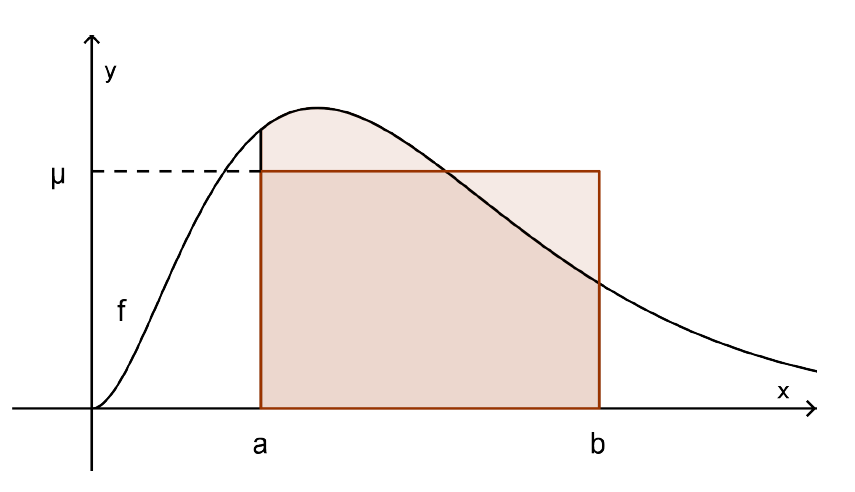
\includegraphics[width=0.4\linewidth]{images/Mittelwert_Grafik.png}
    \end{center}
  Definition des Mittelwert \(\mu\) der Funktion \(f(x)\) auf \([a,b]\): Höhe des Rechtecks, das
  \itemize
    \item eine Grundlinie der Länge \(b-a\) hat
    \item der Flächeninhalt des Rechteks der Fläche unter der Kurve \(f(x)\) im Intervall \([a,b]\) entspricht
	\[\mu = \frac{1}{b-a}\int_a^b{f(x)\mathrm{d}x} \]
\end{theorem}
\begin{formula}{Rotationsvolumen}\\
    \[V = \pi \int_a^b{(f(x))^2\mathrm{d}x} \]
\end{formula}
\begin{formula}{Bogenlänge}\\
    \[L=\int_a^b{\sqrt{1+(f'(x))^2}\mathrm{d}x} \]
\end{formula}
\begin{formula}{Mantelfläche}
    \[M=2\pi \int_a^b{f(x)\cdot \sqrt{1+(f'(x))^2}\mathrm{d}x} \]	
\end{formula}
\begin{theorem}{Schwerpunkt ebener Fläche}\\
  \begin{center}
  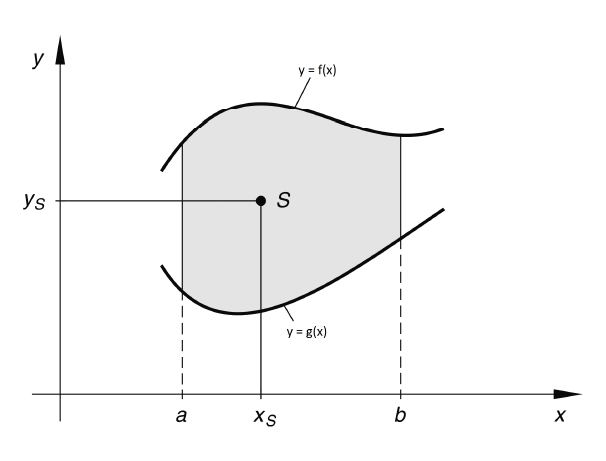
\includegraphics[width=0.4\linewidth]{images/Schwerpunkt_Beispiel.png}
  \end{center}
Schwerpunkt \(S=(x_s;y_s)\) einer ebenen Fläche mit Flächeninhalt A, eingegrenzt von Kurven \(y=f(x)\) und \(y=g(x)\)
sowie den Geraden \(x=a\) und \(x=b\):
\[xs = \frac{1}{A}\int_a^b{x\cdot(f(x)-g(x))\mathrm{d}x} \]
\[ys = \frac{1}{2A}\int_a^b{x\cdot(f(x)^2-g(x)^2)\mathrm{d}x} \]
Berechnen von \(A\) ebenfalls durch ein Integral:
\[A=\int_a^b{f(x)-g(x)\mathrm{d}x} \]
\end{theorem}
\begin{theorem}{Schwerpunkt Rotationskörper}\\
    Die x-Koordinate des Schwerpunkts \(S=(x_s;0;0) \) eines Rotationskörpers mit Volumen \(V\), geformt durch Rotation
    von \(y=f(x)\) zwischen \([a,b]\) um x-Achse mit \(a<b\) und \(f(x) \ge 0 \) für alle \(a \le x \le b \):
    \[x_s = \frac{\pi}{V}\int_a^b{x\cdot f(x)^2\mathrm{d}x} \]
\end{theorem}
